
\section{Visualization System}
As illustrated in Figure~\ref{fig:modelPipeline}, many recent end-to-end NLP model follows a similar encoder, attention, and classifier structure, in which the attention stage provide a window for peeking into the model decision making process. However, the static attention alone likely does not tell the whole story, instead we can learn more about the model by examining the dynamic between the input, the attention, and the output. To allow the user to interrogate the relationship between different components of the pipeline, the proposed system utilizes a perturbation-driven exploration strategy, where the user can manually or automatically perturb the input sentence and then view the aggregated prediction information. Beside the perturbation of the input, the system also allows interactive modification of the attention values, where the prediction will instantaneously updated to reflect the changes. 
%
The system consistence several visualization components that can be combined to generate an functional interactive system. In the following section, we will cover some of the key components.

\subsection{Input Sentences Perturbation}
\label{sec:perturb}
Due to the discrete nature of the natural language, automatically applying perturbation to sentence for sensitivity analysis can be particularly challenging (compared to other domain, i.e., image), as small changes in words can leading to drastic differences in the semantics of the sentences.
To reduce the potential semantic deviation, we first devise a straightforward perturbation method by replacing \emph{nouns} and \emph{verbs} by their synonyms in the wordNet~\cite{Miller1995}. However, the limitation is apparent, as synonyms replacement does not guarantee the meaning of the sentence remain the same. And the wordNet often produces infrequent/obscure usages that may leads to less meaningful perturbed sentences. However, this method requires minimal computation and is easy to implement. 

\begin{figure}[htbp]
\centering
\vspace{-2mm}
 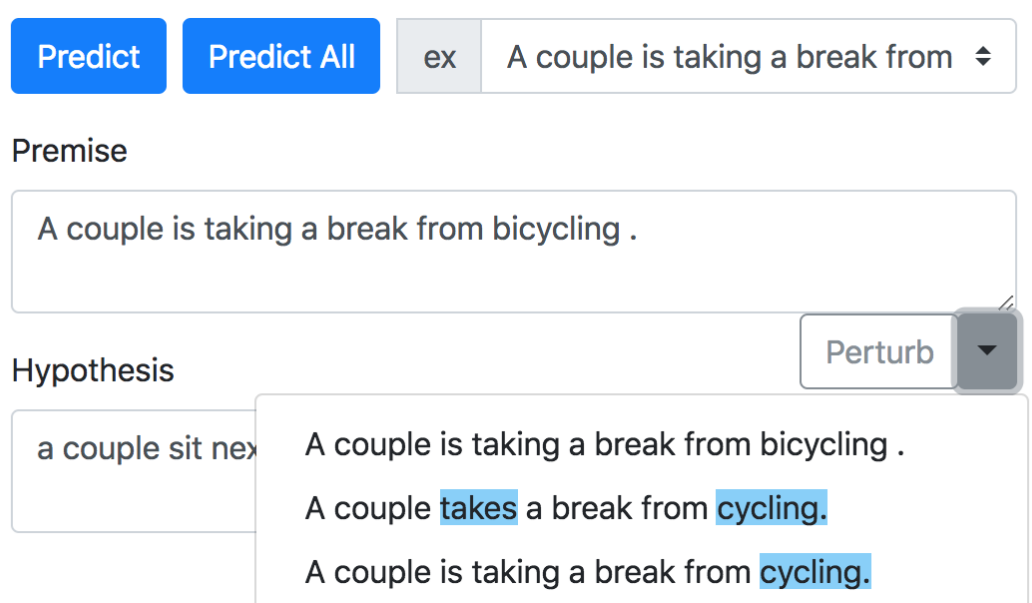
\includegraphics[width=0.9\linewidth]{sentence}
 \vspace{-2mm}
 \caption{
The interface for showing input sentences. The user can manually alter the words or apply automatic perturbation/paraphrasing of the inputs. In the ``perturbed'' dropdown menu, the blue words are the only not exist in the original sentence.
 }
 \vspace{-1mm}
\label{fig:sentence}
\end{figure}

To improve the perturbation quality, we also adopted a translation based paraphrasing technique that is similar to the one discussed in \cite{mallinson2017paraphrasing}. Here, we translate the original English sentence into several other languages and then translate back into English. Provided the translation produce correct result (in our case, we utilized the google cloud translation platform), we essential obtain paraphrasing of the original sentences (see Figure~\ref{fig:sentence}, where the drop-down menu shows the paraphrased/perturbed sentence).

\begin{figure}[htbp]
\centering
\vspace{-2mm}
 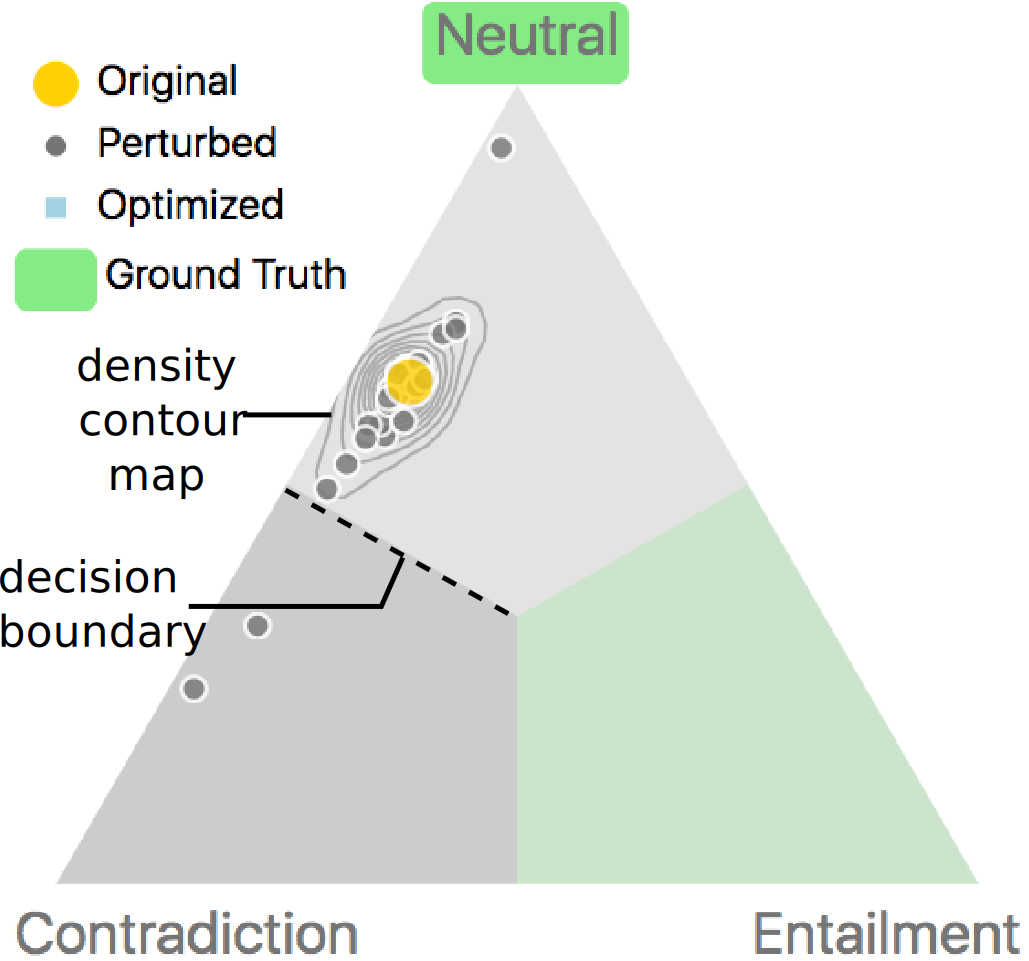
\includegraphics[width=0.8\linewidth]{prediction}
 \caption{
Summarize the prediction results of the perturbed input for the natural language inference model.
the prediction is encoded as a point in the barycentric coordinate system of the triangle, in which each vertex corresponds to one prediction label.
}
\vspace{-3mm}
\label{fig:prediction}
\end{figure}

\subsection{Prediction Visualization}
Efficient visual encoding for prediction is crucial for communicating the model behavior. And to fully support the input perturbation feature, the visual encoding should also allow multiple predictions to be shown in the same visualization.
%
For the natural language inference task, as illustrated in Figure~\ref{fig:prediction}, the predicted probabilities is encoded in the triangle, where the three vertices represents the three possible prediction (namely, \emph{entail}, \emph{contradict}, and \emph{neutral}). The prediction for the original unperturbed input is illustrated by a larger yellow circle, whereas the prediction of perturbed inputs are represented by smaller grey circles.
A density contour of the prediction is computed to emphasize the highly cluttered areas and distinguish the outliers.

\begin{figure*}[t]
\centering
\vspace{-2mm}
 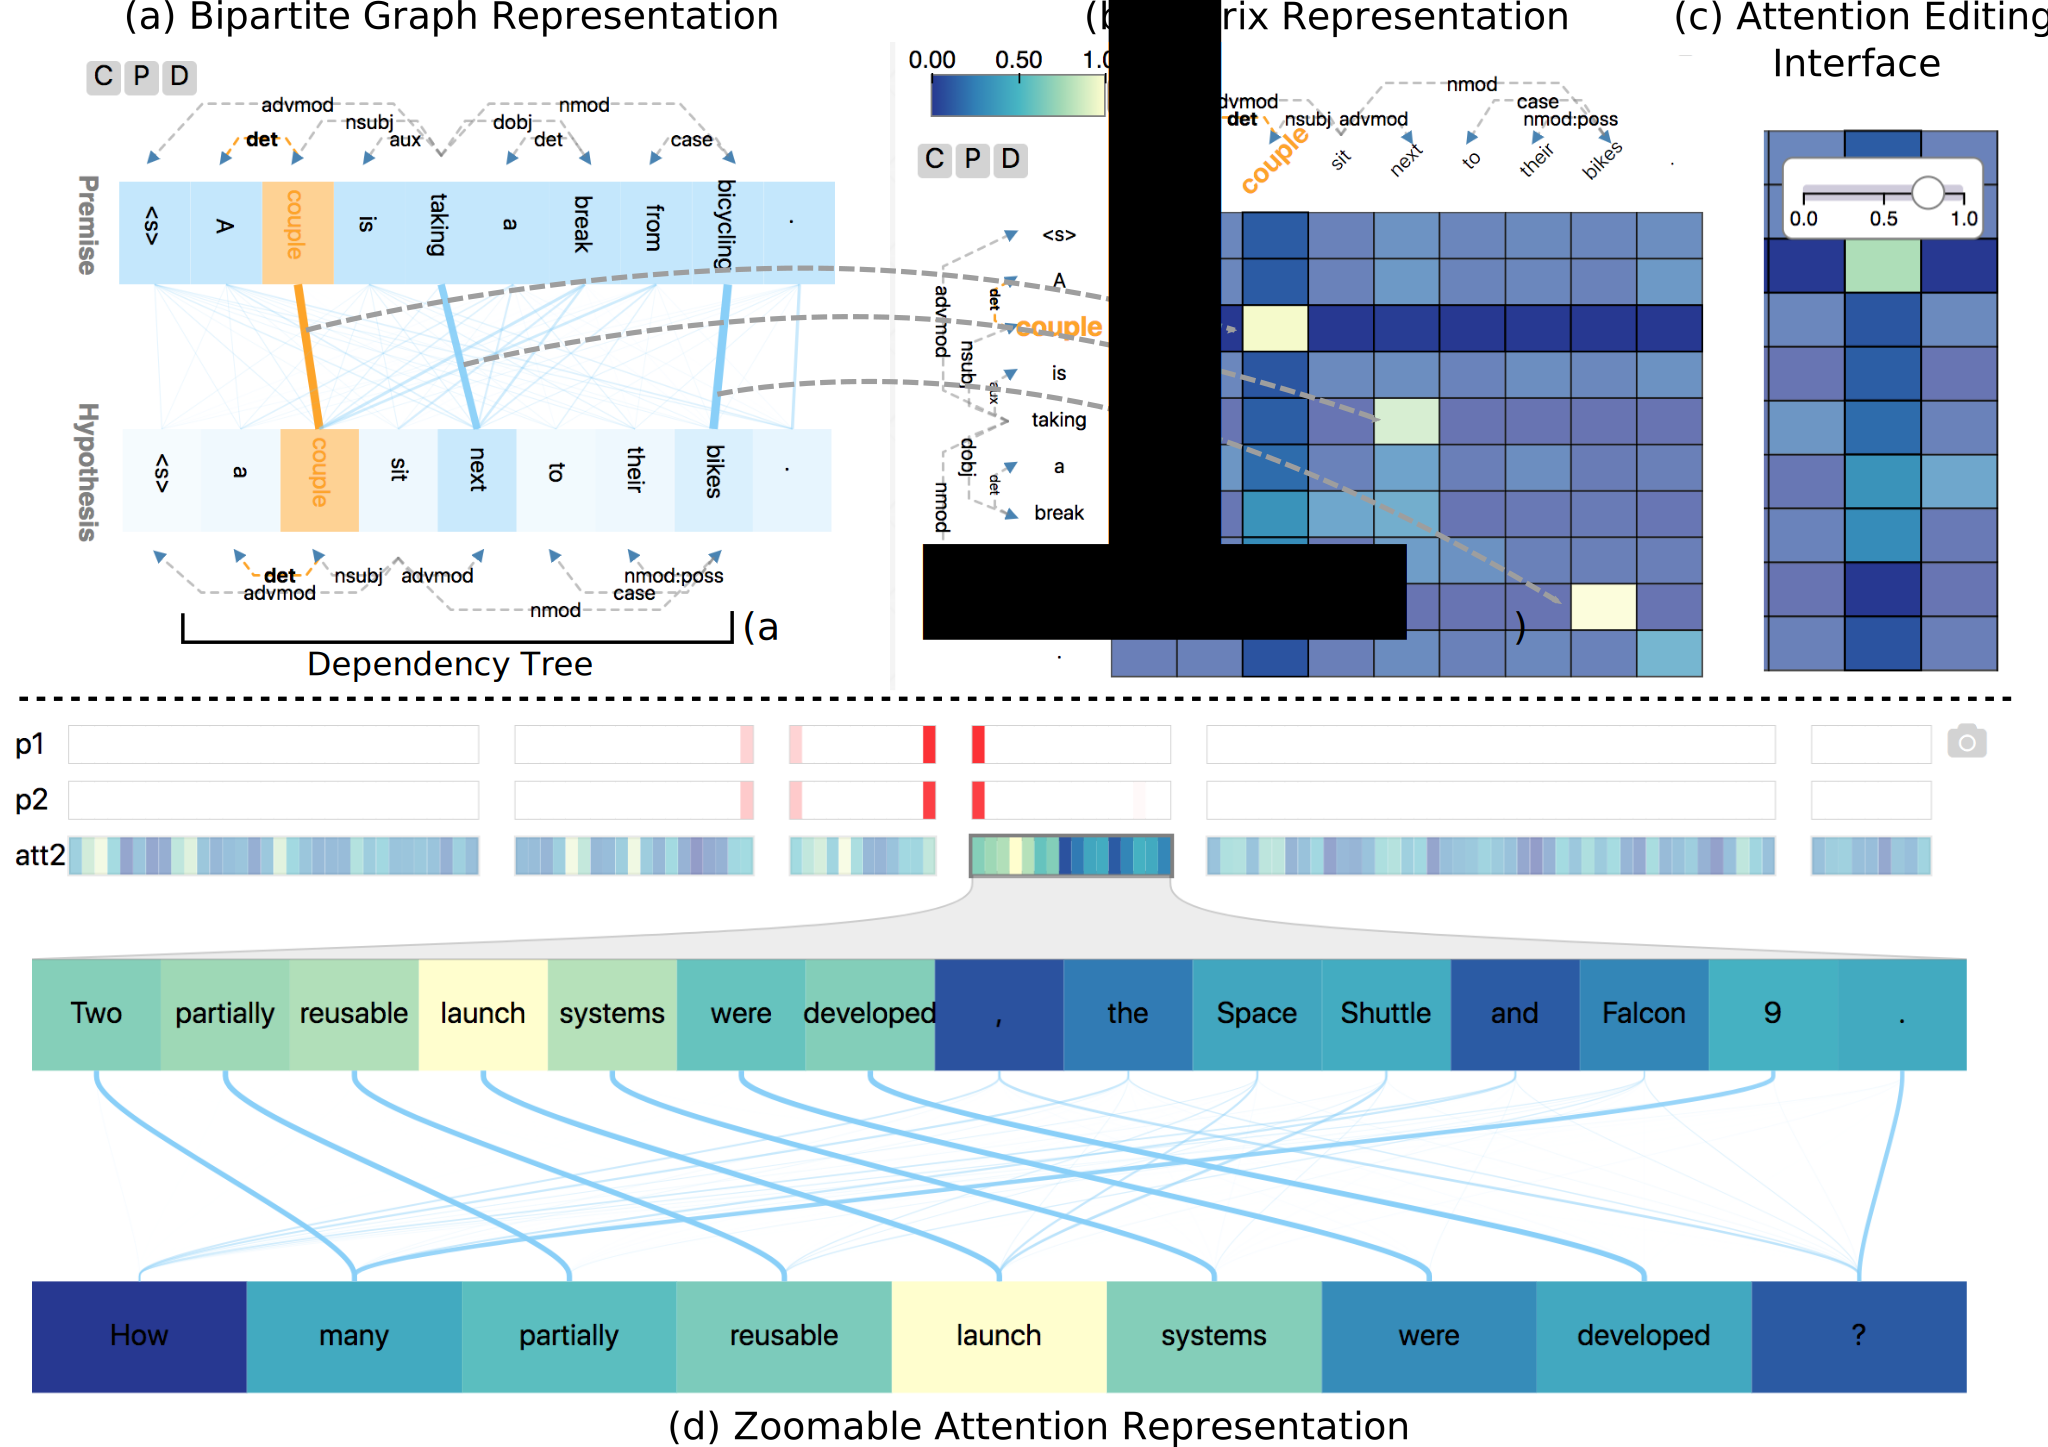
\includegraphics[width=0.95\linewidth]{attentionPanels}
  \vspace{-3mm}
 \caption{
Attention visualization. In the graph attention view (a), a bipartite graph encoding is adopted, in which the edge thickness corresponds to the attention value. In the matrix attention view (b), the entries of $i^{th}$ row represent the probabilities of words in hypotheses align to the $i^{th}$ word in the premise.
The user can alter the attention values via the pop-up interface illustrated in (c).
We overlay the dependency tree ($a_1$) grammar structure to highlight important words and allow simplification of complex sentence based on the dependency tree.
%
For highly asymmetric attention relationship, we utilized a zoomable hierarchical visual representation (d).
}
\vspace{-3mm}
\label{fig:attentionVis}
\end{figure*}

\subsection{Attention Visualization}
As illustrated in Figure~\ref{fig:attentionVis}(a)(b), the most widely adopted technique to bipartie graph (a), as well as the heatmap attention matrix representation (b). 
%
In the graph attention view (Fig.~\ref{fig:attentionVis}(a)), a bipartite graph encoding is adopted, in which the edge thickness corresponds to the attention value. The color of the rectangle text block encodes the sum of all edge values connected to it (darker shade of blues correspond to higher values).
%%%%%%%%
The graph view is suitable for highlighting the most dominant alignments. However, the edges may become cluttered if multiple attention values are high. The matrix attention view (Fig.~\ref{fig:attentionVis}(b)) resolve these issues, despite being more verbose and less efficient in highlighting the dominant alignments. 
We also enable the linkage between highlighted actions in both views (see Fig.~\ref{fig:attentionVis}(a)(b), one the most dominant attention is highlighted in orange).
%
To facilitate the perturbation of attention (see Figure~\ref{fig:modelPipeline}), as illustrated in Figure~\ref{fig:attentionVis}(c), we implement an interface in the matrix view for user to directly manipulate the attention value.

To address the challenge of visualizing long sentence, we augmented the standard visual encoding with grammar structure, and allow dynamic simplification of the sentence based on the dependency tree (see Figure~\ref{fig:attentionVis}(a1)). We also show how the dependency information can potentially improve the prediction result in Section~\ref{sec:NLIexample}

However, when the one of the text sequence become signification longer, i.e., a full paragraph as in the machine comprehension task, the even the simplified sentence can not be meaningfully represented in the graph or matrix visual encoding. To address this visualization challenge, as illustrated in Figure~\ref{fig:attentionVis}(d), we introduce the hierarchical representation. Here, a pure graphical encoding (the color bars marked by \emph{att2}) is used to capture the aggregated alignment information of the whole paragraph, and the user can focus on localized attention information by selecting the a pixel bar that presents a single sentence. We can also link this attention representation with matrix, such that whenever a sentence is selected the local attention relationship is allow shown in the matrix view (see Figure~\ref{fig:MCexample}(a)).

\subsection{Implementation}
The initial setup cost and learning curve of the tool are often the barriers for user adaptation. To address these challenge, we design the visualization system as a Python library with modularity and easy accessibility in mind.
Instead of using the visualization system as a monolithic standalone application, just like a plotting library (i.e., matplotlib), the different pieces of the visualization (i.e., matrix based attention encoding) can be accessed individually.
% 
Yet, the components can also be combined in any configuration desired by users via a simple API to better fit into one's workflow.
More importantly, the library-based design allows easy integration with the existing model implemented in Python.
%
To create a visualization, users only need to import the library, create an instance of the visualization object, and specify a set of callback functions, such as generating a prediction, accessing attention, to link the visualization to their NLP models. The the code required to create an interactive exploration environment for machine comprehension model is illustrated bellow.

\begin{lstlisting}[language=Python, caption=Code for setting up the visualization system shown in Figure~\ref{fig:MCexample}(a).]
from visPackage import MCModule
from bidaf_src import bidafModelInterface
from NLPutility import translationPerturbation

#initialize machine comprehension model
model = bidafModelInterface(
    wordDict="data/bidaf/squad.word.dict",
    wordVec="data/bidaf/glove.hdf5",
    model="data/bidaf/bidaf.ema")
gen = translationPerturbation()
#visualization components
visLayout = {
  "column":[{"row": ["Paragraph", 
                     "AttentionSubMatrix"]},
            {"row": ["AttentionAsymmetric"]}]
  }
#setup interface
modelVis = MCModule(visLayout)
modelVis.setPredictionHook(model.predict)
modelVis.setAttentionHook(model.attention)
modelVis.setSentenceHook(gen.perturbSentence)
#open browser for the web-based visualization
modelVis.show()
\end{lstlisting}




